% %% %%%%%%%%%%%%%%%%%%%%%%%%%%%%%%%%%%%%%%%%%%%%%%%%%%%%%%%%%%
% steps.tex
%
% Author:  Mauricio Matamoros
% License: MIT
%
% %% %%%%%%%%%%%%%%%%%%%%%%%%%%%%%%%%%%%%%%%%%%%%%%%%%%%%%%%%%%
%!TEX root = ../practica.tex
%!TEX root = ../references.bib

% CHKTEX-FILE 1
% CHKTEX-FILE 13
% CHKTEX-FILE 46

\section{Instrucciones}%
\label{sec:instructions}
\begin{enumerate}[noitemsep]
	\item Alambre el circuito de la \href{https://github.com/kyordhel/FSEm/tree/master/practica06}{Práctica 6}.
	\item Alambre el circuito de la \href{https://github.com/kyordhel/FSEm/tree/master/practica07}{Práctica 7}.
	\item Verifique que el sensor de temperatura registra las temperaturas adecuadamente.
	\item Verifique que \emph{dimmer} modula la potencia de la lámpara incandescente adecuadamente.
	\item Integre ambos circuitos e implemente los controladores descritos en las \Cref{sec:step-1,sec:step-2}.
 	\item Realice los experimentos propuestos en la \cref{sec:experiments}.
\end{enumerate}

% %% %%%%%%%%%%%%%%%%%%%%%%%%%%%%%%%%%%%%%%%%%%%%%%%%%%%%%%%%%%
% step-1.tex
%
% Author:  Mauricio Matamoros
% License: MIT
%
% %% %%%%%%%%%%%%%%%%%%%%%%%%%%%%%%%%%%%%%%%%%%%%%%%%%%%%%%%%%%
%!TEX root = ../practica.tex
%!TEX root = ../references.bib

% CHKTEX-FILE 1
% CHKTEX-FILE 13
% CHKTEX-FILE 46

\subsection{Implementación un controlador On/Off}%
\label{sec:step-1}

Alambre cuidadosamente los circuitos de las prácticas \href{https://github.com/kyordhel/FSEm/tree/master/practica06}{6} y \href{https://github.com/kyordhel/FSEm/tree/master/practica07}{7} para crear un circuito AC-DC optoacoplado completo para control cerrado de temperatura usando un foco incandescente operado con un LM35 y un circuito de variación de fase mediante detección de cruce por cero.
El circuito completo alambrado debe verse como el de la \Cref{fig:circuit-full}.

\medskip

\begin{importantbox}{\large Importante}
	\begin{center}
		Asegúrese de verificar con un multímetro que el circuito de AC está debidamente aislado y que no se tienen valores mayores a 5V en el segmento de DC.
		De otro modo podría quemar su Arduino y su Raspberry Pi.
	\end{center}
\end{importantbox}

\medskip

\begin{figure}
	\centering
	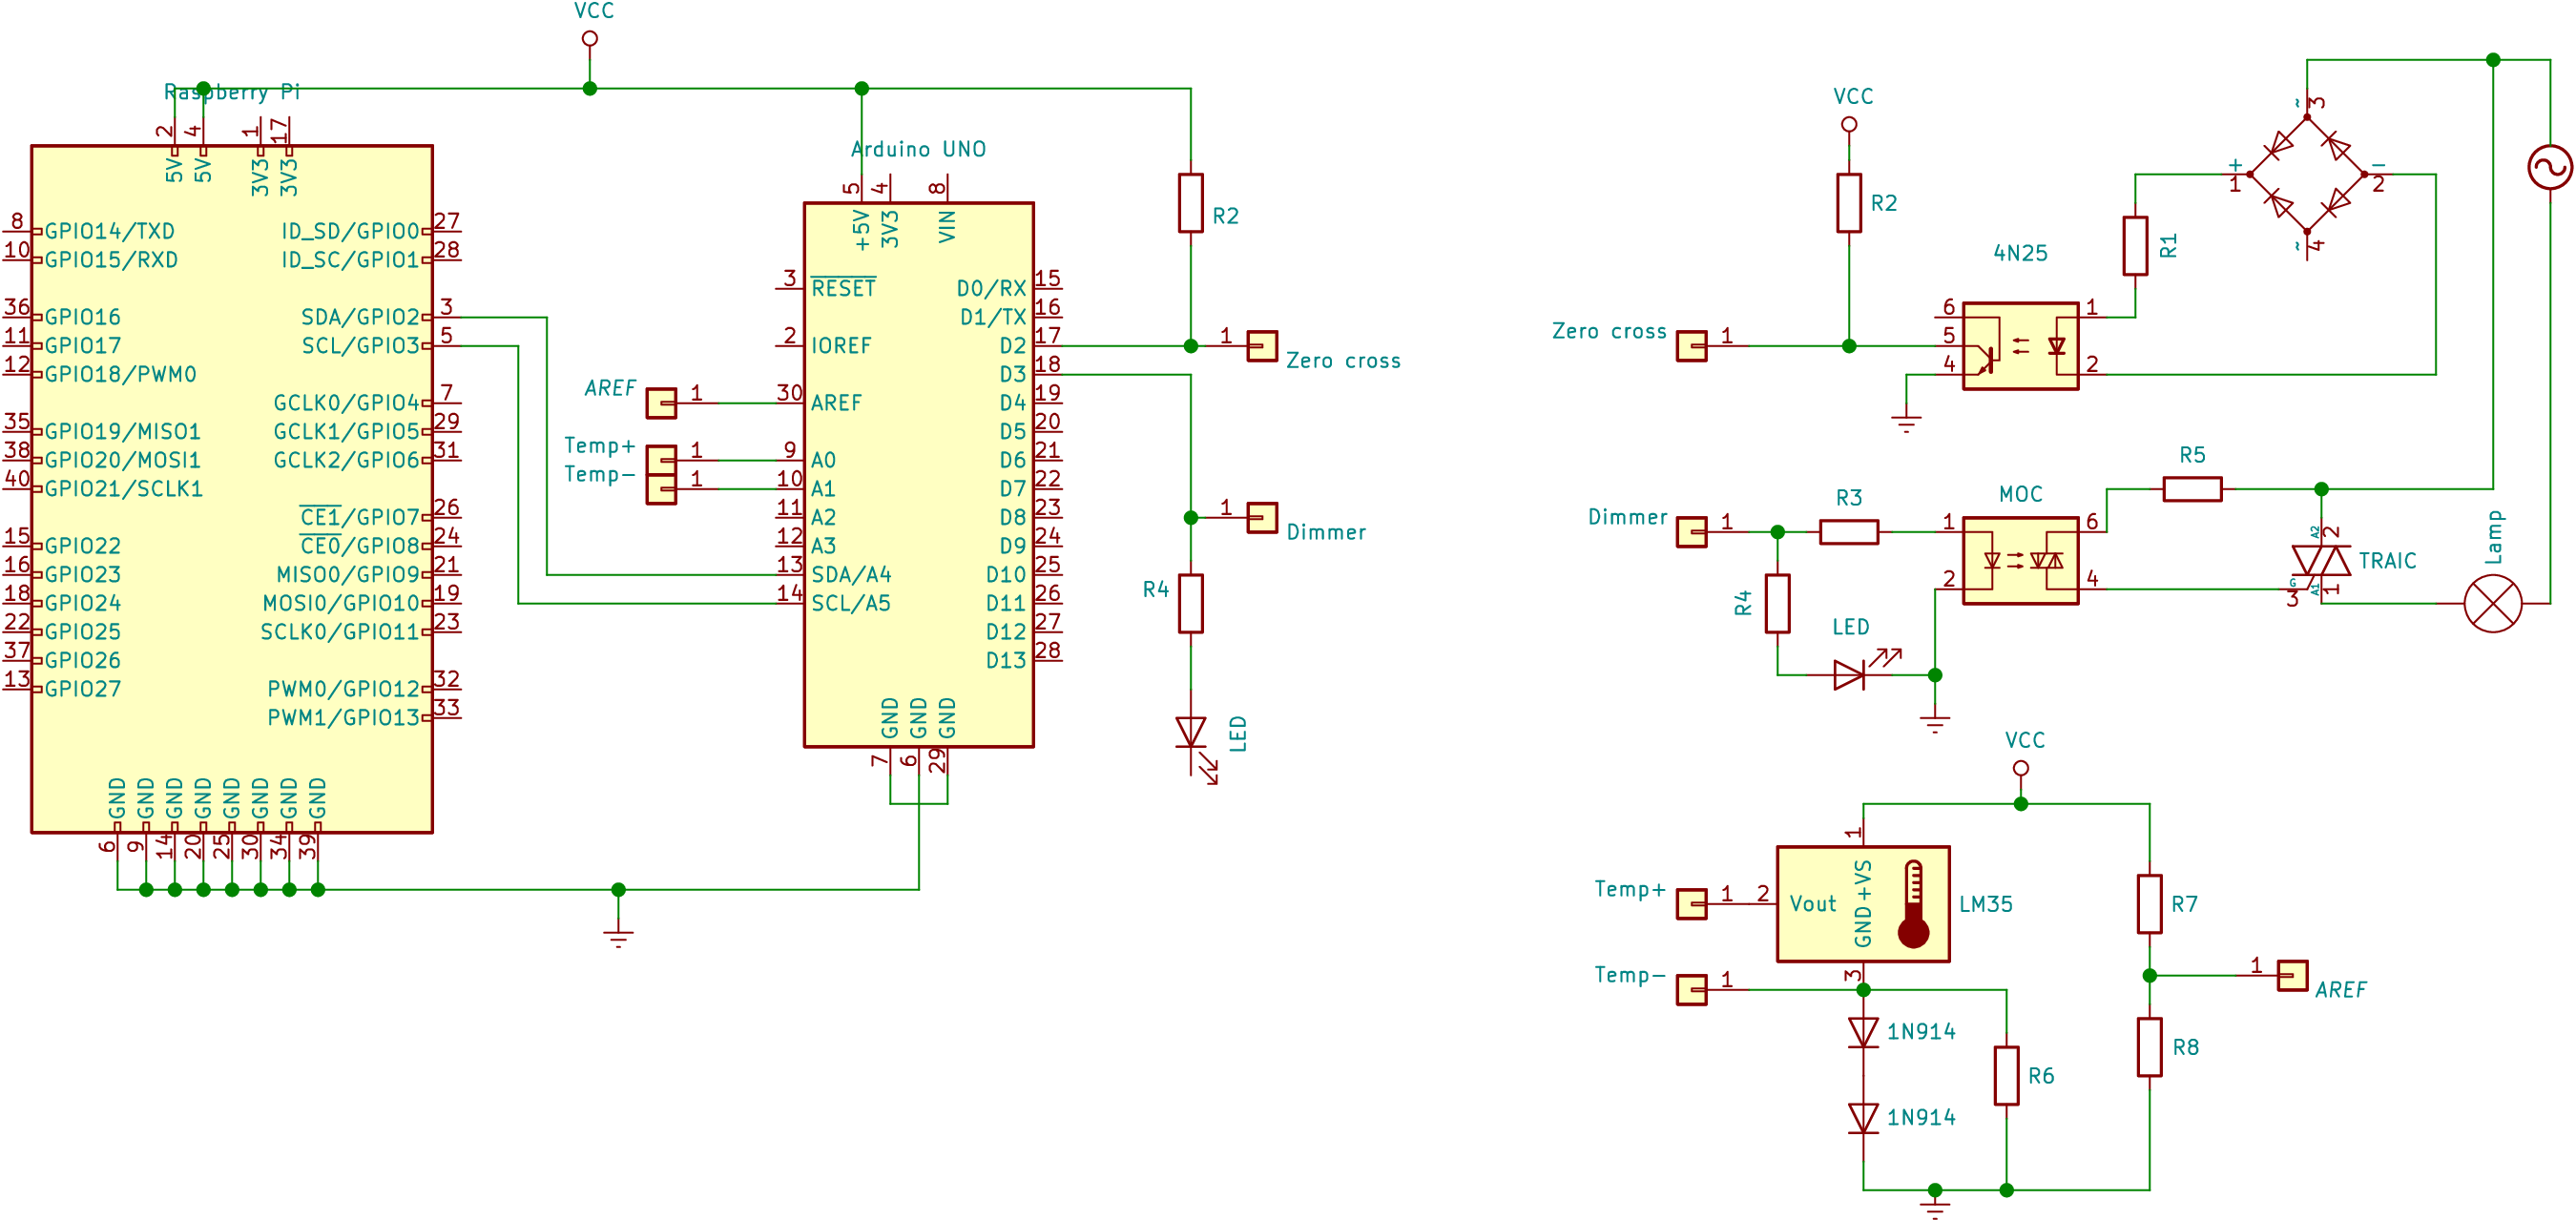
\includegraphics[width=0.85\linewidth,height=6cm,keepaspectratio]{img/circuit-full.png}
	\caption{Circuito AC-DC optoacoplado completo para control cerrado de temperatura.}%
	\label{fig:circuit-full}
\end{figure}

De acuerdo con el alambrado de la \Cref{fig:circuit-full}, el Arduino ha de realizar tres funciones:
\begin{enumerate*}[label=\roman*\rpar]
	\item digitalización del valor de temperatura analógico sensado por el LM35,
	\item la detección del cruce por cero de la onda sinusoidal de la línea eléctrica,
	y
	\item la modulación de potencia del foco incandescente mediante variación de fase ajustada por el retardo en el disparo del TRIAC.
\end{enumerate*}
Al igual que en las prácticas anteriores, el Arduino estará configurado como dispositivo esclavo y estas operaciones estarán al servicio del dispositivo maestro: la Raspberry Pi.
Así, una operación de lectura proporcionará al dispositivo maestro la temperatura sensada, mientras que una operación de escritura enviará la potencia con la que encenderá el foco como un valor flotante entre 0 y 100, quedando a cargo del Arduino el cálculo de la variación de fase y la sincronización de las operaciones de hardware.

\paragraph{Nota:} La implementación del código del Arduino se deja a cargo del estudiante.

\medskip

Se puede proceder entonces a revisar el código de control que se ejecutará en la Raspberry Pi.
En este caso se implementará un controlador On/Off tal como se describe en la \Cref{sec:control-onoff}.

Lo primero es incluir los paquetes necesarios y proveer cuatro parámetros importantes:
\begin{enumerate*}[label=\arabic*\rpar]
	\item la dirección del dispositivo esclavo,
	\item la temperatura deseada,
	\item el umbral o valor de encendido,
	y
	\item el umbral o valor de apagado
\end{enumerate*}
tal como se muestra en el \Cref{lst:controller-code-params}.

\begin{minipage}{\linewidth}%
\lstinputlisting[%
	language=python,
	caption={\texttt{controller-on-off.py:9--20} --- Parámetros},
	label={lst:controller-code-params},
	firstline=9,
	lastline=20]{src/controller-on-off.py}
\end{minipage}

El controlador con los parámetros descritos anteriormente requerirá de dos funciones auxiliares: \emph{readTemperature} (véase \Cref{lst:controller-code-read}) y \emph{writePower} (véase \Cref{lst:controller-code-write}).
La primer función corresponde a una operación de lectura en la cual el Arduino proporcionará la temperatura registrada por el sensor en grados centígrados codificado como un valor flotante (4 bytes en little endian).
La segunda función es una operación de escritura en la cual la Raspberry Pi proporcionará al arduino el factor de potencia de 0 a 100 codificada como un valor flotante (4 bytes en little endian).

\begin{minipage}{\linewidth}%
\lstinputlisting[%
	language=python,
	caption={\texttt{controller-on-off.py:26--36} --- Función \emph{readTemperature}},
	label={lst:controller-code-read},
	firstline=26,
	lastline=36]{src/controller-on-off.py}
\end{minipage}

\begin{minipage}{\linewidth}%
\lstinputlisting[%
	language=python,
	caption={\texttt{controller-on-off.py:38--45} --- Función \emph{writePower}},
	label={lst:controller-code-write},
	firstline=38,
	lastline=45]{src/controller-on-off.py}
\end{minipage}

Por último queda revisar la implementación del controlador mostrada en el \Cref{lst:controller-onoff-code}.
El control de temperatura se ejecuta en un bucle infinito de tres partes dentro de la función principal \emph{main}.
\begin{enumerate*}[label=\arabic*\rpar]
	\item Primero se lee la temperatura en °C del arduino,
	\item después esta se compara con los umbrales.
	Si la temperatura es menor al valor de encendido la lámpara se enciende a máxima potencia y permanecerá encendida hasta que se supera el valor de apagado.
	Por último,
	\item el controlador entra en un estado de espera (1 segundo) donde no se realiza ninguna acción.
\end{enumerate*}
En cualquier otro caso no se hace nada.

\begin{minipage}{\linewidth}%
\lstinputlisting[%
	language=python,
	caption={\texttt{controller-on-off.py:47--67} --- Función \emph{main}},
	label={lst:controller-onoff-code},
	linerange={47-47,51-52,54-55,57-67} %CHKTEX 8
	]{src/controller-on-off.py}
\end{minipage}
% %% %%%%%%%%%%%%%%%%%%%%%%%%%%%%%%%%%%%%%%%%%%%%%%%%%%%%%%%%%%
% step-2.tex
%
% Author:  Mauricio Matamoros
% License: MIT
%
% %% %%%%%%%%%%%%%%%%%%%%%%%%%%%%%%%%%%%%%%%%%%%%%%%%%%%%%%%%%%
%!TEX root = ../practica.tex
%!TEX root = ../references.bib

% CHKTEX-FILE 1
% CHKTEX-FILE 13
% CHKTEX-FILE 46
\subsection{Paso 2: Configuración de comunicaciones \IIC}%
\label{sec:step3}
Primero ha de configurarse la Raspberry Pi para funcionar como dispositivo maestro o \emph{master} en el bus \IIC.
Para esto, inicie la utilidad de configuración de la Raspberry Pi con el comando

\begin{Verbatim}
# raspi-config
\end{Verbatim}

\noindent y seleccione la opción 5: Opciones de Interfaz (\emph{Interfacing Options}) y active la opción \texttt{P5} para habilitar el \IIC.

A continuación, verifique que el puerto \IIC no se encuentre en la lista negra.
Edite el archivo \\\texttt{/etc/modprobe.d/raspi-blacklist.conf} y revise que la línea \texttt{blacklist spi-bcm2708} esté comentada con \#.

% $ cat /etc/modprobe.d/raspi-blacklist.conf
\begin{lstlisting}[
	language=conf,
	caption={/etc/modprobe.d/raspi-blacklist.conf},
	label={lst:raspi-blacklist.conf},
	numbers=none
]
# blacklist spi and i2c by default (many users don't need them)
# blacklist i2c-bcm2708
\end{lstlisting}

Como paso siguiente, se habilita la carga del driver \IIC.
Esto se logra agregando la línea \texttt{i2c-dev} al final del archivo \texttt{/etc/modules} si esta no se encuentra ya allí.

Por último, se instalan los paquetes que permiten la comunicación mediante el bus \IIC y se habilita al usuario predeterminado \emph{pi} (o cualquier otro que se esté usando) para acceder al recurso.

\begin{Verbatim}
# apt-get install i2c-tools python-smbus
# adduser pi i2c
\end{Verbatim}

Reinicie la Raspberry Pi y pruebe la configuración ejecutando \texttt{i2cdetect -y 1} para buscar dispositivos conectados al bus \IIC.
Debería ver una salida como la siguiente:

\begin{Verbatim}
\$ i2cdetect -y 1
     0  1  2  3  4  5  6  7  8  9  a  b  c  d  e  f
00:          -- -- -- -- -- -- -- -- -- -- -- --
10: -- -- -- -- -- -- -- -- -- -- -- -- -- -- --
20: -- -- -- -- -- -- -- -- -- -- -- -- -- -- --
30: -- -- -- -- -- -- -- -- -- -- -- -- -- -- --
40: -- -- -- -- -- -- -- -- -- -- -- -- -- -- --
50: -- -- -- -- -- -- -- -- -- -- -- -- -- -- --
60: -- -- -- -- -- -- -- -- -- -- -- -- -- -- --
70: -- -- -- -- -- -- -- --
\end{Verbatim}

% % %% %%%%%%%%%%%%%%%%%%%%%%%%%%%%%%%%%%%%%%%%%%%%%%%%%%%%%%%%%%
% step-3.tex
%
% Author:  Mauricio Matamoros
% License: MIT
%
% %% %%%%%%%%%%%%%%%%%%%%%%%%%%%%%%%%%%%%%%%%%%%%%%%%%%%%%%%%%%

%!TEX root = ../main.tex
%!TEX root = ../references.bib

\subsection{Paso 3: Display de siete segmentos}%
\label{sec:step4}
El código mostrado en \Cref{src:bcd} muestra cómo se operaría un display de siete segmentos mediante una controladora TTL 74LS47 utilizando la Raspberry Pi.

\smallskip
\lstinputlisting[%
	language=Python,
	linerange={19-51}, % chktex 8
	caption={\texttt{bcd.py}},
	label={src:bcd}
]{src/bcd.py}
\smallskip

Estudie el código y véalo en funcionamiento, ejecutándolo de la siguiente manera:
\begin{Verbatim}[fontsize=\footnotesize]
./bcd.py
\end{Verbatim}






